\documentclass[1p]{elsarticle_modified}
%\bibliographystyle{elsarticle-num}

%\usepackage[colorlinks]{hyperref}
%\usepackage{abbrmath_seonhwa} %\Abb, \Ascr, \Acal ,\Abf, \Afrak
\usepackage{amsfonts}
\usepackage{amssymb}
\usepackage{amsmath}
\usepackage{amsthm}
\usepackage{scalefnt}
\usepackage{amsbsy}
\usepackage{kotex}
\usepackage{caption}
\usepackage{subfig}
\usepackage{color}
\usepackage{graphicx}
\usepackage{xcolor} %% white, black, red, green, blue, cyan, magenta, yellow
\usepackage{float}
\usepackage{setspace}
\usepackage{hyperref}

\usepackage{tikz}
\usetikzlibrary{arrows}

\usepackage{multirow}
\usepackage{array} % fixed length table
\usepackage{hhline}

%%%%%%%%%%%%%%%%%%%%%
\makeatletter
\renewcommand*\env@matrix[1][\arraystretch]{%
	\edef\arraystretch{#1}%
	\hskip -\arraycolsep
	\let\@ifnextchar\new@ifnextchar
	\array{*\c@MaxMatrixCols c}}
\makeatother %https://tex.stackexchange.com/questions/14071/how-can-i-increase-the-line-spacing-in-a-matrix
%%%%%%%%%%%%%%%

\usepackage[normalem]{ulem}

\newcommand{\msout}[1]{\ifmmode\text{\sout{\ensuremath{#1}}}\else\sout{#1}\fi}
%SOURCE: \msout is \stkout macro in https://tex.stackexchange.com/questions/20609/strikeout-in-math-mode

\newcommand{\cancel}[1]{
	\ifmmode
	{\color{red}\msout{#1}}
	\else
	{\color{red}\sout{#1}}
	\fi
}

\newcommand{\add}[1]{
	{\color{blue}\uwave{#1}}
}

\newcommand{\replace}[2]{
	\ifmmode
	{\color{red}\msout{#1}}{\color{blue}\uwave{#2}}
	\else
	{\color{red}\sout{#1}}{\color{blue}\uwave{#2}}
	\fi
}

\newcommand{\Sol}{\mathcal{S}} %segment
\newcommand{\D}{D} %diagram
\newcommand{\A}{\mathcal{A}} %arc


%%%%%%%%%%%%%%%%%%%%%%%%%%%%%5 test

\def\sl{\operatorname{\textup{SL}}(2,\Cbb)}
\def\psl{\operatorname{\textup{PSL}}(2,\Cbb)}
\def\quan{\mkern 1mu \triangleright \mkern 1mu}

\theoremstyle{definition}
\newtheorem{thm}{Theorem}[section]
\newtheorem{prop}[thm]{Proposition}
\newtheorem{lem}[thm]{Lemma}
\newtheorem{ques}[thm]{Question}
\newtheorem{cor}[thm]{Corollary}
\newtheorem{defn}[thm]{Definition}
\newtheorem{exam}[thm]{Example}
\newtheorem{rmk}[thm]{Remark}
\newtheorem{alg}[thm]{Algorithm}

\newcommand{\I}{\sqrt{-1}}
\begin{document}

%\begin{frontmatter}
%
%\title{Boundary parabolic representations of knots up to 8 crossings}
%
%%% Group authors per affiliation:
%\author{Yunhi Cho} 
%\address{Department of Mathematics, University of Seoul, Seoul, Korea}
%\ead{yhcho@uos.ac.kr}
%
%
%\author{Seonhwa Kim} %\fnref{s_kim}}
%\address{Center for Geometry and Physics, Institute for Basic Science, Pohang, 37673, Korea}
%\ead{ryeona17@ibs.re.kr}
%
%\author{Hyuk Kim}
%\address{Department of Mathematical Sciences, Seoul National University, Seoul 08826, Korea}
%\ead{hyukkim@snu.ac.kr}
%
%\author{Seokbeom Yoon}
%\address{Department of Mathematical Sciences, Seoul National University, Seoul, 08826,  Korea}
%\ead{sbyoon15@snu.ac.kr}
%
%\begin{abstract}
%We find all boundary parabolic representation of knots up to 8 crossings.
%
%\end{abstract}
%\begin{keyword}
%    \MSC[2010] 57M25 
%\end{keyword}
%
%\end{frontmatter}

%\linenumbers
%\tableofcontents
%
\newcommand\colored[1]{\textcolor{white}{\rule[-0.35ex]{0.8em}{1.4ex}}\kern-0.8em\color{red} #1}%
%\newcommand\colored[1]{\textcolor{white}{ #1}\kern-2.17ex	\textcolor{white}{ #1}\kern-1.81ex	\textcolor{white}{ #1}\kern-2.15ex\color{red}#1	}

{\Large $\underline{12a_{0861}~(K12a_{0861})}$}

\setlength{\tabcolsep}{10pt}
\renewcommand{\arraystretch}{1.6}
\vspace{1cm}\begin{tabular}{m{100pt}>{\centering\arraybackslash}m{274pt}}
\multirow{5}{120pt}{
	\centering
	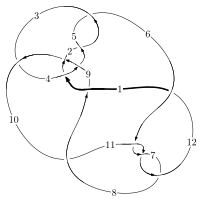
\includegraphics[width=112pt]{../../../GIT/diagram.site/Diagrams/png/1662_12a_0861.png}\\
\ \ \ A knot diagram\footnotemark}&
\allowdisplaybreaks
\textbf{Linearized knot diagam} \\
\cline{2-2}
 &
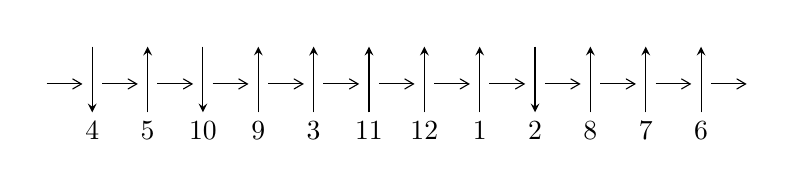
\begin{tikzpicture}[x=20pt, y=17pt]
	% nodes
	\node (C0) at (0, 0) {};
	\node (C1) at (1, 0) {};
	\node (C1U) at (1, +1) {};
	\node (C1D) at (1, -1) {4};

	\node (C2) at (2, 0) {};
	\node (C2U) at (2, +1) {};
	\node (C2D) at (2, -1) {5};

	\node (C3) at (3, 0) {};
	\node (C3U) at (3, +1) {};
	\node (C3D) at (3, -1) {10};

	\node (C4) at (4, 0) {};
	\node (C4U) at (4, +1) {};
	\node (C4D) at (4, -1) {9};

	\node (C5) at (5, 0) {};
	\node (C5U) at (5, +1) {};
	\node (C5D) at (5, -1) {3};

	\node (C6) at (6, 0) {};
	\node (C6U) at (6, +1) {};
	\node (C6D) at (6, -1) {11};

	\node (C7) at (7, 0) {};
	\node (C7U) at (7, +1) {};
	\node (C7D) at (7, -1) {12};

	\node (C8) at (8, 0) {};
	\node (C8U) at (8, +1) {};
	\node (C8D) at (8, -1) {1};

	\node (C9) at (9, 0) {};
	\node (C9U) at (9, +1) {};
	\node (C9D) at (9, -1) {2};

	\node (C10) at (10, 0) {};
	\node (C10U) at (10, +1) {};
	\node (C10D) at (10, -1) {8};

	\node (C11) at (11, 0) {};
	\node (C11U) at (11, +1) {};
	\node (C11D) at (11, -1) {7};

	\node (C12) at (12, 0) {};
	\node (C12U) at (12, +1) {};
	\node (C12D) at (12, -1) {6};
	\node (C13) at (13, 0) {};

	% arrows
	\draw[->,>={angle 60}]
	(C0) edge (C1) (C1) edge (C2) (C2) edge (C3) (C3) edge (C4) (C4) edge (C5) (C5) edge (C6) (C6) edge (C7) (C7) edge (C8) (C8) edge (C9) (C9) edge (C10) (C10) edge (C11) (C11) edge (C12) (C12) edge (C13) ;	\draw[->,>=stealth]
	(C1U) edge (C1D) (C2D) edge (C2U) (C3U) edge (C3D) (C4D) edge (C4U) (C5D) edge (C5U) (C6D) edge (C6U) (C7D) edge (C7U) (C8D) edge (C8U) (C9U) edge (C9D) (C10D) edge (C10U) (C11D) edge (C11U) (C12D) edge (C12U) ;
	\end{tikzpicture} \\
\hhline{~~} \\& 
\textbf{Solving Sequence} \\ \cline{2-2} 
 &
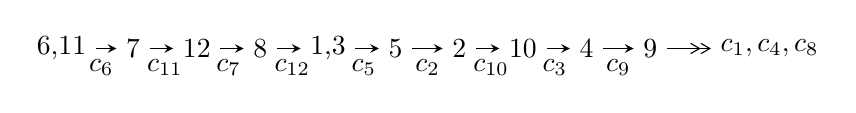
\begin{tikzpicture}[x=23pt, y=7pt]
	% node
	\node (A0) at (-1/8, 0) {6,11};
	\node (A1) at (1, 0) {7};
	\node (A2) at (2, 0) {12};
	\node (A3) at (3, 0) {8};
	\node (A4) at (65/16, 0) {1,3};
	\node (A5) at (41/8, 0) {5};
	\node (A6) at (49/8, 0) {2};
	\node (A7) at (57/8, 0) {10};
	\node (A8) at (65/8, 0) {4};
	\node (A9) at (73/8, 0) {9};
	\node (C1) at (1/2, -1) {$c_{6}$};
	\node (C2) at (3/2, -1) {$c_{11}$};
	\node (C3) at (5/2, -1) {$c_{7}$};
	\node (C4) at (7/2, -1) {$c_{12}$};
	\node (C5) at (37/8, -1) {$c_{5}$};
	\node (C6) at (45/8, -1) {$c_{2}$};
	\node (C7) at (53/8, -1) {$c_{10}$};
	\node (C8) at (61/8, -1) {$c_{3}$};
	\node (C9) at (69/8, -1) {$c_{9}$};
	\node (A10) at (11, 0) {$c_{1},c_{4},c_{8}$};

	% edge
	\draw[->,>=stealth]	
	(A0) edge (A1) (A1) edge (A2) (A2) edge (A3) (A3) edge (A4) (A4) edge (A5) (A5) edge (A6) (A6) edge (A7) (A7) edge (A8) (A8) edge (A9) ;
	\draw[->>,>={angle 60}]	
	(A9) edge (A10);
\end{tikzpicture} \\ 

\end{tabular} \\

\footnotetext{
The image of knot diagram is generated by the software ``\textbf{Draw programme}" developed by Andrew Bartholomew(\url{http://www.layer8.co.uk/maths/draw/index.htm\#Running-draw}), where we modified some parts for our purpose(\url{https://github.com/CATsTAILs/LinksPainter}).
}\phantom \\ \newline 
\centering \textbf{Ideals for irreducible components\footnotemark of $X_{\text{par}}$} 
 
\begin{align*}
I^u_{1}&=\langle 
-1.81318\times10^{32} u^{100}-1.67567\times10^{32} u^{99}+\cdots+8.39034\times10^{32} b+8.52545\times10^{32},\\
\phantom{I^u_{1}}&\phantom{= \langle  }-1.89290\times10^{31} u^{100}+3.18867\times10^{32} u^{99}+\cdots+4.19517\times10^{32} a+4.50214\times10^{32},\\
\phantom{I^u_{1}}&\phantom{= \langle  }u^{101}+2 u^{100}+\cdots-5 u-1\rangle \\
I^u_{2}&=\langle 
b-1,\;a+1,\;u+1\rangle \\
\\
\end{align*}
\raggedright * 2 irreducible components of $\dim_{\mathbb{C}}=0$, with total 102 representations.\\
\footnotetext{All coefficients of polynomials are rational numbers. But the coefficients are sometimes approximated in decimal forms when there is not enough margin.}
\newpage
\renewcommand{\arraystretch}{1}
\centering \section*{I. $I^u_{1}= \langle -1.81\times10^{32} u^{100}-1.68\times10^{32} u^{99}+\cdots+8.39\times10^{32} b+8.53\times10^{32},\;-1.89\times10^{31} u^{100}+3.19\times10^{32} u^{99}+\cdots+4.20\times10^{32} a+4.50\times10^{32},\;u^{101}+2 u^{100}+\cdots-5 u-1 \rangle$}
\flushleft \textbf{(i) Arc colorings}\\
\begin{tabular}{m{7pt} m{180pt} m{7pt} m{180pt} }
\flushright $a_{6}=$&$\begin{pmatrix}1\\0\end{pmatrix}$ \\
\flushright $a_{11}=$&$\begin{pmatrix}0\\u\end{pmatrix}$ \\
\flushright $a_{7}=$&$\begin{pmatrix}1\\- u^2\end{pmatrix}$ \\
\flushright $a_{12}=$&$\begin{pmatrix}u\\- u^3+u\end{pmatrix}$ \\
\flushright $a_{8}=$&$\begin{pmatrix}- u^2+1\\u^4-2 u^2\end{pmatrix}$ \\
\flushright $a_{1}=$&$\begin{pmatrix}- u^3+2 u\\- u^3+u\end{pmatrix}$ \\
\flushright $a_{3}=$&$\begin{pmatrix}0.0451209 u^{100}-0.760082 u^{99}+\cdots+9.26245 u-1.07317\\0.216103 u^{100}+0.199714 u^{99}+\cdots-0.0924635 u-1.01610\end{pmatrix}$ \\
\flushright $a_{5}=$&$\begin{pmatrix}-0.0356196 u^{100}+0.759959 u^{99}+\cdots-10.8577 u+1.72341\\-0.135588 u^{100}-0.201144 u^{99}+\cdots-0.369854 u+0.935588\end{pmatrix}$ \\
\flushright $a_{2}=$&$\begin{pmatrix}0.197101 u^{100}+0.199959 u^{99}+\cdots-5.90190 u-0.316585\\0.838970 u^{100}+0.00285885 u^{99}+\cdots-4.07536 u-0.838970\end{pmatrix}$ \\
\flushright $a_{10}=$&$\begin{pmatrix}- u^5+2 u^3- u\\u^7-3 u^5+2 u^3+u\end{pmatrix}$ \\
\flushright $a_{4}=$&$\begin{pmatrix}0.0393835 u^{100}-0.759997 u^{99}+\cdots+9.26178 u-1.07334\\-1.33209 u^{100}-1.40778 u^{99}+\cdots+8.49440 u+1.33209\end{pmatrix}$ \\
\flushright $a_{9}=$&$\begin{pmatrix}u^{10}-5 u^8+8 u^6-3 u^4-3 u^2+1\\u^{10}-4 u^8+5 u^6-3 u^2\end{pmatrix}$\\&\end{tabular}
\flushleft \textbf{(ii) Obstruction class $= -1$}\\~\\
\flushleft \textbf{(iii) Cusp Shapes $= -2.45932 u^{100}+4.76034 u^{99}+\cdots+0.110956 u+1.41932$}\\~\\
\newpage\renewcommand{\arraystretch}{1}
\flushleft \textbf{(iv) u-Polynomials at the component}\newline \\
\begin{tabular}{m{50pt}|m{274pt}}
Crossings & \hspace{64pt}u-Polynomials at each crossing \\
\hline $$\begin{aligned}c_{1}\end{aligned}$$&$\begin{aligned}
&u^{101}-17 u^{100}+\cdots+2 u+2
\end{aligned}$\\
\hline $$\begin{aligned}c_{2},c_{5}\end{aligned}$$&$\begin{aligned}
&u^{101}+2 u^{100}+\cdots-13 u+1
\end{aligned}$\\
\hline $$\begin{aligned}c_{3}\end{aligned}$$&$\begin{aligned}
&u^{101}+2 u^{100}+\cdots-365721 u+33833
\end{aligned}$\\
\hline $$\begin{aligned}c_{4}\end{aligned}$$&$\begin{aligned}
&u^{101}+4 u^{100}+\cdots+8829 u+2851
\end{aligned}$\\
\hline $$\begin{aligned}c_{6},c_{7},c_{11}\end{aligned}$$&$\begin{aligned}
&u^{101}-2 u^{100}+\cdots-5 u+1
\end{aligned}$\\
\hline $$\begin{aligned}c_{8}\end{aligned}$$&$\begin{aligned}
&u^{101}-24 u^{99}+\cdots-140961 u+15661
\end{aligned}$\\
\hline $$\begin{aligned}c_{9}\end{aligned}$$&$\begin{aligned}
&u^{101}-4 u^{100}+\cdots- u+1
\end{aligned}$\\
\hline $$\begin{aligned}c_{10},c_{12}\end{aligned}$$&$\begin{aligned}
&u^{101}+3 u^{100}+\cdots-133 u^2+32
\end{aligned}$\\
\hline
\end{tabular}\\~\\
\newpage\renewcommand{\arraystretch}{1}
\flushleft \textbf{(v) Riley Polynomials at the component}\newline \\
\begin{tabular}{m{50pt}|m{274pt}}
Crossings & \hspace{64pt}Riley Polynomials at each crossing \\
\hline $$\begin{aligned}c_{1}\end{aligned}$$&$\begin{aligned}
&y^{101}+9 y^{100}+\cdots-56 y-4
\end{aligned}$\\
\hline $$\begin{aligned}c_{2},c_{5}\end{aligned}$$&$\begin{aligned}
&y^{101}-72 y^{100}+\cdots- y-1
\end{aligned}$\\
\hline $$\begin{aligned}c_{3}\end{aligned}$$&$\begin{aligned}
&y^{101}-68 y^{100}+\cdots-23745298781 y-1144671889
\end{aligned}$\\
\hline $$\begin{aligned}c_{4}\end{aligned}$$&$\begin{aligned}
&y^{101}-120 y^{100}+\cdots+659640771 y-8128201
\end{aligned}$\\
\hline $$\begin{aligned}c_{6},c_{7},c_{11}\end{aligned}$$&$\begin{aligned}
&y^{101}-84 y^{100}+\cdots- y-1
\end{aligned}$\\
\hline $$\begin{aligned}c_{8}\end{aligned}$$&$\begin{aligned}
&y^{101}-48 y^{100}+\cdots-5147347709 y-245266921
\end{aligned}$\\
\hline $$\begin{aligned}c_{9}\end{aligned}$$&$\begin{aligned}
&y^{101}+16 y^{100}+\cdots- y-1
\end{aligned}$\\
\hline $$\begin{aligned}c_{10},c_{12}\end{aligned}$$&$\begin{aligned}
&y^{101}+57 y^{100}+\cdots+8512 y-1024
\end{aligned}$\\
\hline
\end{tabular}\\~\\
\newpage\flushleft \textbf{(vi) Complex Volumes and Cusp Shapes}
$$\begin{array}{c|c|c}  
\text{Solutions to }I^u_{1}& \I (\text{vol} + \sqrt{-1}CS) & \text{Cusp shape}\\
 \hline 
\begin{aligned}
u &= -1.028940 + 0.386413 I \\
a &= \phantom{-}0.0973768 + 0.0686506 I \\
b &= \phantom{-}1.104430 + 0.134470 I\end{aligned}
 & \phantom{-}3.30551 + 1.15808 I & \phantom{-0.000000 } 0 \\ \hline\begin{aligned}
u &= -1.028940 - 0.386413 I \\
a &= \phantom{-}0.0973768 - 0.0686506 I \\
b &= \phantom{-}1.104430 - 0.134470 I\end{aligned}
 & \phantom{-}3.30551 - 1.15808 I & \phantom{-0.000000 } 0 \\ \hline\begin{aligned}
u &= \phantom{-}1.057030 + 0.349481 I \\
a &= \phantom{-}0.314048 - 0.736272 I \\
b &= \phantom{-}1.36678 - 0.53207 I\end{aligned}
 & \phantom{-}4.49153 - 9.62146 I & \phantom{-0.000000 } 0 \\ \hline\begin{aligned}
u &= \phantom{-}1.057030 - 0.349481 I \\
a &= \phantom{-}0.314048 + 0.736272 I \\
b &= \phantom{-}1.36678 + 0.53207 I\end{aligned}
 & \phantom{-}4.49153 + 9.62146 I & \phantom{-0.000000 } 0 \\ \hline\begin{aligned}
u &= \phantom{-}1.111270 + 0.222770 I \\
a &= -0.366060 + 0.901400 I \\
b &= -1.32169 + 0.64309 I\end{aligned}
 & \phantom{-}4.72151 - 1.48890 I & \phantom{-0.000000 } 0 \\ \hline\begin{aligned}
u &= \phantom{-}1.111270 - 0.222770 I \\
a &= -0.366060 - 0.901400 I \\
b &= -1.32169 - 0.64309 I\end{aligned}
 & \phantom{-}4.72151 + 1.48890 I & \phantom{-0.000000 } 0 \\ \hline\begin{aligned}
u &= \phantom{-}1.099330 + 0.300902 I \\
a &= -0.188576 + 1.200930 I \\
b &= -0.002327 + 1.136800 I\end{aligned}
 & \phantom{-}0.17070 - 3.78814 I & \phantom{-0.000000 } 0 \\ \hline\begin{aligned}
u &= \phantom{-}1.099330 - 0.300902 I \\
a &= -0.188576 - 1.200930 I \\
b &= -0.002327 - 1.136800 I\end{aligned}
 & \phantom{-}0.17070 + 3.78814 I & \phantom{-0.000000 } 0 \\ \hline\begin{aligned}
u &= -0.173926 + 0.812684 I \\
a &= \phantom{-}0.73131 - 1.40433 I \\
b &= \phantom{-}1.142840 - 0.188317 I\end{aligned}
 & \phantom{-}0.67914 - 5.50977 I & \phantom{-}8.94619 + 9.47296 I \\ \hline\begin{aligned}
u &= -0.173926 - 0.812684 I \\
a &= \phantom{-}0.73131 + 1.40433 I \\
b &= \phantom{-}1.142840 + 0.188317 I\end{aligned}
 & \phantom{-}0.67914 + 5.50977 I & \phantom{-}8.94619 - 9.47296 I\\
 \hline 
 \end{array}$$\newpage$$\begin{array}{c|c|c}  
\text{Solutions to }I^u_{1}& \I (\text{vol} + \sqrt{-1}CS) & \text{Cusp shape}\\
 \hline 
\begin{aligned}
u &= -1.17114\phantom{ +0.000000I} \\
a &= -0.989252\phantom{ +0.000000I} \\
b &= \phantom{-}0.346774\phantom{ +0.000000I}\end{aligned}
 & \phantom{-}2.12529\phantom{ +0.000000I} & \phantom{-0.000000 } 0 \\ \hline\begin{aligned}
u &= -0.025467 + 0.828000 I \\
a &= \phantom{-}1.60890 - 1.16076 I \\
b &= \phantom{-}1.063360 - 0.411521 I\end{aligned}
 & -3.81109 - 5.30422 I & \phantom{-}2.34656 + 6.94530 I \\ \hline\begin{aligned}
u &= -0.025467 - 0.828000 I \\
a &= \phantom{-}1.60890 + 1.16076 I \\
b &= \phantom{-}1.063360 + 0.411521 I\end{aligned}
 & -3.81109 + 5.30422 I & \phantom{-}2.34656 - 6.94530 I \\ \hline\begin{aligned}
u &= \phantom{-}0.158631 + 0.804073 I \\
a &= \phantom{-}0.80609 + 2.49041 I \\
b &= \phantom{-}1.38917 + 0.54718 I\end{aligned}
 & \phantom{-}1.74695 + 13.85140 I & \phantom{-}6.00000 - 8.73084 I \\ \hline\begin{aligned}
u &= \phantom{-}0.158631 - 0.804073 I \\
a &= \phantom{-}0.80609 - 2.49041 I \\
b &= \phantom{-}1.38917 - 0.54718 I\end{aligned}
 & \phantom{-}1.74695 - 13.85140 I & \phantom{-}6.00000 + 8.73084 I \\ \hline\begin{aligned}
u &= -1.149270 + 0.299595 I \\
a &= -0.542737 - 0.500847 I \\
b &= \phantom{-}0.057454 - 0.251125 I\end{aligned}
 & \phantom{-}0.654538 - 0.558503 I & \phantom{-0.000000 } 0 \\ \hline\begin{aligned}
u &= -1.149270 - 0.299595 I \\
a &= -0.542737 + 0.500847 I \\
b &= \phantom{-}0.057454 + 0.251125 I\end{aligned}
 & \phantom{-}0.654538 + 0.558503 I & \phantom{-0.000000 } 0 \\ \hline\begin{aligned}
u &= -1.165090 + 0.250717 I \\
a &= \phantom{-}1.93078 - 2.43537 I \\
b &= -1.031870 - 0.085936 I\end{aligned}
 & \phantom{-}2.90707 - 0.81510 I & \phantom{-0.000000 } 0 \\ \hline\begin{aligned}
u &= -1.165090 - 0.250717 I \\
a &= \phantom{-}1.93078 + 2.43537 I \\
b &= -1.031870 + 0.085936 I\end{aligned}
 & \phantom{-}2.90707 + 0.81510 I & \phantom{-0.000000 } 0 \\ \hline\begin{aligned}
u &= -0.667105 + 0.437770 I \\
a &= \phantom{-}0.059804 - 0.895514 I \\
b &= \phantom{-}1.150220 - 0.000851 I\end{aligned}
 & \phantom{-}4.39007 - 0.66689 I & \phantom{-}20.5536 + 2.2015 I\\
 \hline 
 \end{array}$$\newpage$$\begin{array}{c|c|c}  
\text{Solutions to }I^u_{1}& \I (\text{vol} + \sqrt{-1}CS) & \text{Cusp shape}\\
 \hline 
\begin{aligned}
u &= -0.667105 - 0.437770 I \\
a &= \phantom{-}0.059804 + 0.895514 I \\
b &= \phantom{-}1.150220 + 0.000851 I\end{aligned}
 & \phantom{-}4.39007 + 0.66689 I & \phantom{-}20.5536 - 2.2015 I \\ \hline\begin{aligned}
u &= \phantom{-}0.138798 + 0.781657 I \\
a &= \phantom{-}0.95689 - 2.16420 I \\
b &= -0.028732 - 1.197250 I\end{aligned}
 & -2.72320 + 7.79519 I & \phantom{-}3.29744 - 8.41863 I \\ \hline\begin{aligned}
u &= \phantom{-}0.138798 - 0.781657 I \\
a &= \phantom{-}0.95689 + 2.16420 I \\
b &= -0.028732 + 1.197250 I\end{aligned}
 & -2.72320 - 7.79519 I & \phantom{-}3.29744 + 8.41863 I \\ \hline\begin{aligned}
u &= -0.116871 + 0.774426 I \\
a &= -0.234715 + 0.892659 I \\
b &= -0.002107 + 0.327040 I\end{aligned}
 & -2.44866 - 3.37818 I & \phantom{-}2.29820 + 1.98806 I \\ \hline\begin{aligned}
u &= -0.116871 - 0.774426 I \\
a &= -0.234715 - 0.892659 I \\
b &= -0.002107 - 0.327040 I\end{aligned}
 & -2.44866 + 3.37818 I & \phantom{-}2.29820 - 1.98806 I \\ \hline\begin{aligned}
u &= \phantom{-}0.022502 + 0.782527 I \\
a &= \phantom{-}0.00177 + 2.09029 I \\
b &= \phantom{-}0.377607 + 0.784247 I\end{aligned}
 & -5.93645 - 0.87720 I & -1.80763 + 1.04585 I \\ \hline\begin{aligned}
u &= \phantom{-}0.022502 - 0.782527 I \\
a &= \phantom{-}0.00177 - 2.09029 I \\
b &= \phantom{-}0.377607 - 0.784247 I\end{aligned}
 & -5.93645 + 0.87720 I & -1.80763 - 1.04585 I \\ \hline\begin{aligned}
u &= \phantom{-}1.209230 + 0.196168 I \\
a &= \phantom{-}0.119207 - 0.751916 I \\
b &= -1.46666 - 0.24510 I\end{aligned}
 & \phantom{-}5.39958 + 2.00182 I & \phantom{-0.000000 } 0 \\ \hline\begin{aligned}
u &= \phantom{-}1.209230 - 0.196168 I \\
a &= \phantom{-}0.119207 + 0.751916 I \\
b &= -1.46666 + 0.24510 I\end{aligned}
 & \phantom{-}5.39958 - 2.00182 I & \phantom{-0.000000 } 0 \\ \hline\begin{aligned}
u &= \phantom{-}0.144908 + 0.752921 I \\
a &= -0.80543 - 2.77881 I \\
b &= -1.41125 - 0.69668 I\end{aligned}
 & \phantom{-}1.90392 + 5.20096 I & \phantom{-}9.90636 - 7.40698 I\\
 \hline 
 \end{array}$$\newpage$$\begin{array}{c|c|c}  
\text{Solutions to }I^u_{1}& \I (\text{vol} + \sqrt{-1}CS) & \text{Cusp shape}\\
 \hline 
\begin{aligned}
u &= \phantom{-}0.144908 - 0.752921 I \\
a &= -0.80543 + 2.77881 I \\
b &= -1.41125 + 0.69668 I\end{aligned}
 & \phantom{-}1.90392 - 5.20096 I & \phantom{-}9.90636 + 7.40698 I \\ \hline\begin{aligned}
u &= -0.122529 + 0.744900 I \\
a &= \phantom{-}1.28109 + 2.64200 I \\
b &= -1.076030 + 0.080017 I\end{aligned}
 & -0.16683 - 2.84840 I & -10.9682 - 9.6416 I \\ \hline\begin{aligned}
u &= -0.122529 - 0.744900 I \\
a &= \phantom{-}1.28109 - 2.64200 I \\
b &= -1.076030 - 0.080017 I\end{aligned}
 & -0.16683 + 2.84840 I & -10.9682 + 9.6416 I \\ \hline\begin{aligned}
u &= -1.215600 + 0.269888 I \\
a &= -1.22265 + 2.30397 I \\
b &= -0.753849 + 0.101521 I\end{aligned}
 & \phantom{-}2.23401 - 1.72679 I & \phantom{-0.000000 } 0 \\ \hline\begin{aligned}
u &= -1.215600 - 0.269888 I \\
a &= -1.22265 - 2.30397 I \\
b &= -0.753849 - 0.101521 I\end{aligned}
 & \phantom{-}2.23401 + 1.72679 I & \phantom{-0.000000 } 0 \\ \hline\begin{aligned}
u &= \phantom{-}0.663413 + 0.357602 I \\
a &= -0.39860 + 1.58817 I \\
b &= \phantom{-}1.36297 + 0.47360 I\end{aligned}
 & \phantom{-}5.38362 + 9.52573 I & \phantom{-}10.14946 - 8.06140 I \\ \hline\begin{aligned}
u &= \phantom{-}0.663413 - 0.357602 I \\
a &= -0.39860 - 1.58817 I \\
b &= \phantom{-}1.36297 - 0.47360 I\end{aligned}
 & \phantom{-}5.38362 - 9.52573 I & \phantom{-}10.14946 + 8.06140 I \\ \hline\begin{aligned}
u &= \phantom{-}0.142148 + 0.718668 I \\
a &= -1.70541 - 0.45845 I \\
b &= -1.55105 + 0.40005 I\end{aligned}
 & \phantom{-}2.42332 + 1.28126 I & \phantom{-}11.19302 - 1.21201 I \\ \hline\begin{aligned}
u &= \phantom{-}0.142148 - 0.718668 I \\
a &= -1.70541 + 0.45845 I \\
b &= -1.55105 - 0.40005 I\end{aligned}
 & \phantom{-}2.42332 - 1.28126 I & \phantom{-}11.19302 + 1.21201 I \\ \hline\begin{aligned}
u &= -0.086682 + 0.719986 I \\
a &= -1.87211 - 1.11449 I \\
b &= -0.607902 - 0.121137 I\end{aligned}
 & -1.19230 - 1.84846 I & \phantom{-}5.59881 + 5.60914 I\\
 \hline 
 \end{array}$$\newpage$$\begin{array}{c|c|c}  
\text{Solutions to }I^u_{1}& \I (\text{vol} + \sqrt{-1}CS) & \text{Cusp shape}\\
 \hline 
\begin{aligned}
u &= -0.086682 - 0.719986 I \\
a &= -1.87211 + 1.11449 I \\
b &= -0.607902 + 0.121137 I\end{aligned}
 & -1.19230 + 1.84846 I & \phantom{-}5.59881 - 5.60914 I \\ \hline\begin{aligned}
u &= -0.328118 + 0.635795 I \\
a &= \phantom{-}0.587168 - 0.849188 I \\
b &= \phantom{-}1.180890 - 0.101731 I\end{aligned}
 & \phantom{-}3.33957 - 3.21650 I & \phantom{-}13.9460 + 8.2744 I \\ \hline\begin{aligned}
u &= -0.328118 - 0.635795 I \\
a &= \phantom{-}0.587168 + 0.849188 I \\
b &= \phantom{-}1.180890 + 0.101731 I\end{aligned}
 & \phantom{-}3.33957 + 3.21650 I & \phantom{-}13.9460 - 8.2744 I \\ \hline\begin{aligned}
u &= \phantom{-}1.241200 + 0.334119 I \\
a &= \phantom{-}0.360958 - 1.070060 I \\
b &= \phantom{-}0.328687 - 0.849373 I\end{aligned}
 & -2.17713 + 4.90687 I & \phantom{-0.000000 } 0 \\ \hline\begin{aligned}
u &= \phantom{-}1.241200 - 0.334119 I \\
a &= \phantom{-}0.360958 + 1.070060 I \\
b &= \phantom{-}0.328687 + 0.849373 I\end{aligned}
 & -2.17713 - 4.90687 I & \phantom{-0.000000 } 0 \\ \hline\begin{aligned}
u &= \phantom{-}1.258760 + 0.261311 I \\
a &= -0.388419 - 1.268170 I \\
b &= -0.712654 - 0.731199 I\end{aligned}
 & \phantom{-}2.95981 + 4.71416 I & \phantom{-0.000000 } 0 \\ \hline\begin{aligned}
u &= \phantom{-}1.258760 - 0.261311 I \\
a &= -0.388419 + 1.268170 I \\
b &= -0.712654 + 0.731199 I\end{aligned}
 & \phantom{-}2.95981 - 4.71416 I & \phantom{-0.000000 } 0 \\ \hline\begin{aligned}
u &= -1.232030 + 0.377233 I \\
a &= \phantom{-}0.864114 - 0.126972 I \\
b &= \phantom{-}1.023920 + 0.365529 I\end{aligned}
 & -0.086339 + 0.972263 I & \phantom{-0.000000 } 0 \\ \hline\begin{aligned}
u &= -1.232030 - 0.377233 I \\
a &= \phantom{-}0.864114 + 0.126972 I \\
b &= \phantom{-}1.023920 - 0.365529 I\end{aligned}
 & -0.086339 - 0.972263 I & \phantom{-0.000000 } 0 \\ \hline\begin{aligned}
u &= \phantom{-}0.267208 + 0.647741 I \\
a &= \phantom{-}1.074640 + 0.156641 I \\
b &= \phantom{-}1.348860 - 0.415383 I\end{aligned}
 & \phantom{-}4.04661 - 5.89569 I & \phantom{-}8.02593 + 2.38848 I\\
 \hline 
 \end{array}$$\newpage$$\begin{array}{c|c|c}  
\text{Solutions to }I^u_{1}& \I (\text{vol} + \sqrt{-1}CS) & \text{Cusp shape}\\
 \hline 
\begin{aligned}
u &= \phantom{-}0.267208 - 0.647741 I \\
a &= \phantom{-}1.074640 - 0.156641 I \\
b &= \phantom{-}1.348860 + 0.415383 I\end{aligned}
 & \phantom{-}4.04661 + 5.89569 I & \phantom{-}8.02593 - 2.38848 I \\ \hline\begin{aligned}
u &= -1.277780 + 0.336776 I \\
a &= -0.96889 - 1.44778 I \\
b &= \phantom{-}0.432231 - 0.726486 I\end{aligned}
 & -1.89447 - 3.15775 I & \phantom{-0.000000 } 0 \\ \hline\begin{aligned}
u &= -1.277780 - 0.336776 I \\
a &= -0.96889 + 1.44778 I \\
b &= \phantom{-}0.432231 + 0.726486 I\end{aligned}
 & -1.89447 + 3.15775 I & \phantom{-0.000000 } 0 \\ \hline\begin{aligned}
u &= \phantom{-}1.276690 + 0.370859 I \\
a &= \phantom{-}0.24342 + 1.58444 I \\
b &= \phantom{-}1.101580 + 0.445043 I\end{aligned}
 & \phantom{-}0.23553 + 9.61140 I & \phantom{-0.000000 } 0 \\ \hline\begin{aligned}
u &= \phantom{-}1.276690 - 0.370859 I \\
a &= \phantom{-}0.24342 - 1.58444 I \\
b &= \phantom{-}1.101580 - 0.445043 I\end{aligned}
 & \phantom{-}0.23553 - 9.61140 I & \phantom{-0.000000 } 0 \\ \hline\begin{aligned}
u &= \phantom{-}0.655925 + 0.092614 I \\
a &= \phantom{-}0.605869 - 0.934639 I \\
b &= -1.41714 - 0.52149 I\end{aligned}
 & \phantom{-}4.79133 + 1.83073 I & \phantom{-}15.9174 - 4.3853 I \\ \hline\begin{aligned}
u &= \phantom{-}0.655925 - 0.092614 I \\
a &= \phantom{-}0.605869 + 0.934639 I \\
b &= -1.41714 + 0.52149 I\end{aligned}
 & \phantom{-}4.79133 - 1.83073 I & \phantom{-}15.9174 + 4.3853 I \\ \hline\begin{aligned}
u &= \phantom{-}0.083312 + 0.638423 I \\
a &= -1.52776 + 1.29828 I \\
b &= -0.393511 + 0.804360 I\end{aligned}
 & -0.78660 - 1.45210 I & \phantom{-}4.75717 + 3.49284 I \\ \hline\begin{aligned}
u &= \phantom{-}0.083312 - 0.638423 I \\
a &= -1.52776 - 1.29828 I \\
b &= -0.393511 - 0.804360 I\end{aligned}
 & -0.78660 + 1.45210 I & \phantom{-}4.75717 - 3.49284 I \\ \hline\begin{aligned}
u &= \phantom{-}1.327260 + 0.305233 I \\
a &= -0.999324 + 0.544062 I \\
b &= -0.544745 + 0.207352 I\end{aligned}
 & \phantom{-}3.26237 + 5.56922 I & \phantom{-0.000000 } 0\\
 \hline 
 \end{array}$$\newpage$$\begin{array}{c|c|c}  
\text{Solutions to }I^u_{1}& \I (\text{vol} + \sqrt{-1}CS) & \text{Cusp shape}\\
 \hline 
\begin{aligned}
u &= \phantom{-}1.327260 - 0.305233 I \\
a &= -0.999324 - 0.544062 I \\
b &= -0.544745 - 0.207352 I\end{aligned}
 & \phantom{-}3.26237 - 5.56922 I & \phantom{-0.000000 } 0 \\ \hline\begin{aligned}
u &= -1.333400 + 0.285277 I \\
a &= -1.308200 + 0.029554 I \\
b &= -0.417099 - 1.003450 I\end{aligned}
 & \phantom{-}3.72956 - 1.98995 I & \phantom{-0.000000 } 0 \\ \hline\begin{aligned}
u &= -1.333400 - 0.285277 I \\
a &= -1.308200 - 0.029554 I \\
b &= -0.417099 + 1.003450 I\end{aligned}
 & \phantom{-}3.72956 + 1.98995 I & \phantom{-0.000000 } 0 \\ \hline\begin{aligned}
u &= \phantom{-}0.584196 + 0.241797 I \\
a &= \phantom{-}0.514031 - 0.720592 I \\
b &= -0.111711 - 1.036120 I\end{aligned}
 & \phantom{-}0.79560 + 4.22285 I & \phantom{-}8.17162 - 8.18777 I \\ \hline\begin{aligned}
u &= \phantom{-}0.584196 - 0.241797 I \\
a &= \phantom{-}0.514031 + 0.720592 I \\
b &= -0.111711 + 1.036120 I\end{aligned}
 & \phantom{-}0.79560 - 4.22285 I & \phantom{-}8.17162 + 8.18777 I \\ \hline\begin{aligned}
u &= \phantom{-}1.373580 + 0.023066 I \\
a &= -0.371764 - 0.485397 I \\
b &= -0.245715 - 0.271745 I\end{aligned}
 & \phantom{-}6.80271 + 0.87572 I & \phantom{-0.000000 } 0 \\ \hline\begin{aligned}
u &= \phantom{-}1.373580 - 0.023066 I \\
a &= -0.371764 + 0.485397 I \\
b &= -0.245715 + 0.271745 I\end{aligned}
 & \phantom{-}6.80271 - 0.87572 I & \phantom{-0.000000 } 0 \\ \hline\begin{aligned}
u &= \phantom{-}1.341270 + 0.317191 I \\
a &= \phantom{-}2.53148 - 2.64892 I \\
b &= -1.099120 - 0.079524 I\end{aligned}
 & \phantom{-}4.44329 + 6.70063 I & \phantom{-0.000000 } 0 \\ \hline\begin{aligned}
u &= \phantom{-}1.341270 - 0.317191 I \\
a &= \phantom{-}2.53148 + 2.64892 I \\
b &= -1.099120 + 0.079524 I\end{aligned}
 & \phantom{-}4.44329 - 6.70063 I & \phantom{-0.000000 } 0 \\ \hline\begin{aligned}
u &= \phantom{-}1.340190 + 0.331849 I \\
a &= -0.007094 - 0.596349 I \\
b &= -0.035880 - 0.370722 I\end{aligned}
 & \phantom{-}2.13625 + 7.37812 I & \phantom{-0.000000 } 0\\
 \hline 
 \end{array}$$\newpage$$\begin{array}{c|c|c}  
\text{Solutions to }I^u_{1}& \I (\text{vol} + \sqrt{-1}CS) & \text{Cusp shape}\\
 \hline 
\begin{aligned}
u &= \phantom{-}1.340190 - 0.331849 I \\
a &= -0.007094 + 0.596349 I \\
b &= -0.035880 + 0.370722 I\end{aligned}
 & \phantom{-}2.13625 - 7.37812 I & \phantom{-0.000000 } 0 \\ \hline\begin{aligned}
u &= \phantom{-}1.38147\phantom{ +0.000000I} \\
a &= \phantom{-}4.13434\phantom{ +0.000000I} \\
b &= -1.10712\phantom{ +0.000000I}\end{aligned}
 & \phantom{-}8.57526\phantom{ +0.000000I} & \phantom{-0.000000 } 0 \\ \hline\begin{aligned}
u &= -1.347990 + 0.305884 I \\
a &= \phantom{-}0.05456 + 1.56249 I \\
b &= -1.60063 - 0.43183 I\end{aligned}
 & \phantom{-}7.12028 - 5.01369 I & \phantom{-0.000000 } 0 \\ \hline\begin{aligned}
u &= -1.347990 - 0.305884 I \\
a &= \phantom{-}0.05456 - 1.56249 I \\
b &= -1.60063 + 0.43183 I\end{aligned}
 & \phantom{-}7.12028 + 5.01369 I & \phantom{-0.000000 } 0 \\ \hline\begin{aligned}
u &= -1.351550 + 0.319734 I \\
a &= \phantom{-}1.18973 + 2.47107 I \\
b &= -1.44983 + 0.71711 I\end{aligned}
 & \phantom{-}6.62110 - 9.09012 I & \phantom{-0.000000 } 0 \\ \hline\begin{aligned}
u &= -1.351550 - 0.319734 I \\
a &= \phantom{-}1.18973 - 2.47107 I \\
b &= -1.44983 - 0.71711 I\end{aligned}
 & \phantom{-}6.62110 + 9.09012 I & \phantom{-0.000000 } 0 \\ \hline\begin{aligned}
u &= -1.351170 + 0.333884 I \\
a &= \phantom{-}1.53027 + 0.79665 I \\
b &= -0.046975 + 1.229100 I\end{aligned}
 & \phantom{-}1.97105 - 11.82780 I & \phantom{-0.000000 } 0 \\ \hline\begin{aligned}
u &= -1.351170 - 0.333884 I \\
a &= \phantom{-}1.53027 - 0.79665 I \\
b &= -0.046975 - 1.229100 I\end{aligned}
 & \phantom{-}1.97105 + 11.82780 I & \phantom{-0.000000 } 0 \\ \hline\begin{aligned}
u &= -1.391490 + 0.034086 I \\
a &= \phantom{-}0.403840 - 0.401540 I \\
b &= -0.192149 + 1.152040 I\end{aligned}
 & \phantom{-}6.87246 - 4.91775 I & \phantom{-0.000000 } 0 \\ \hline\begin{aligned}
u &= -1.391490 - 0.034086 I \\
a &= \phantom{-}0.403840 + 0.401540 I \\
b &= -0.192149 - 1.152040 I\end{aligned}
 & \phantom{-}6.87246 + 4.91775 I & \phantom{-0.000000 } 0\\
 \hline 
 \end{array}$$\newpage$$\begin{array}{c|c|c}  
\text{Solutions to }I^u_{1}& \I (\text{vol} + \sqrt{-1}CS) & \text{Cusp shape}\\
 \hline 
\begin{aligned}
u &= -1.395780 + 0.009794 I \\
a &= \phantom{-}1.88400 + 0.12574 I \\
b &= -1.53124 + 0.58610 I\end{aligned}
 & \phantom{-}10.97350 - 2.04434 I & \phantom{-0.000000 } 0 \\ \hline\begin{aligned}
u &= -1.395780 - 0.009794 I \\
a &= \phantom{-}1.88400 - 0.12574 I \\
b &= -1.53124 - 0.58610 I\end{aligned}
 & \phantom{-}10.97350 + 2.04434 I & \phantom{-0.000000 } 0 \\ \hline\begin{aligned}
u &= -1.375500 + 0.257636 I \\
a &= -0.577498 - 0.904908 I \\
b &= \phantom{-}1.38751 + 0.38451 I\end{aligned}
 & \phantom{-}9.21390 + 2.61600 I & \phantom{-0.000000 } 0 \\ \hline\begin{aligned}
u &= -1.375500 - 0.257636 I \\
a &= -0.577498 + 0.904908 I \\
b &= \phantom{-}1.38751 - 0.38451 I\end{aligned}
 & \phantom{-}9.21390 - 2.61600 I & \phantom{-0.000000 } 0 \\ \hline\begin{aligned}
u &= \phantom{-}1.385100 + 0.240167 I \\
a &= -0.892088 + 0.865446 I \\
b &= \phantom{-}1.269340 + 0.115116 I\end{aligned}
 & \phantom{-}8.72575 + 6.33979 I & \phantom{-0.000000 } 0 \\ \hline\begin{aligned}
u &= \phantom{-}1.385100 - 0.240167 I \\
a &= -0.892088 - 0.865446 I \\
b &= \phantom{-}1.269340 - 0.115116 I\end{aligned}
 & \phantom{-}8.72575 - 6.33979 I & \phantom{-0.000000 } 0 \\ \hline\begin{aligned}
u &= -1.363820 + 0.343210 I \\
a &= -0.96059 - 2.44773 I \\
b &= \phantom{-}1.40458 - 0.55203 I\end{aligned}
 & \phantom{-}6.5501 - 17.9931 I & \phantom{-0.000000 } 0 \\ \hline\begin{aligned}
u &= -1.363820 - 0.343210 I \\
a &= -0.96059 + 2.44773 I \\
b &= \phantom{-}1.40458 + 0.55203 I\end{aligned}
 & \phantom{-}6.5501 + 17.9931 I & \phantom{-0.000000 } 0 \\ \hline\begin{aligned}
u &= \phantom{-}1.37172 + 0.34509 I \\
a &= -0.59183 + 1.70310 I \\
b &= \phantom{-}1.176520 + 0.206396 I\end{aligned}
 & \phantom{-}5.55962 + 9.68623 I & \phantom{-0.000000 } 0 \\ \hline\begin{aligned}
u &= \phantom{-}1.37172 - 0.34509 I \\
a &= -0.59183 - 1.70310 I \\
b &= \phantom{-}1.176520 - 0.206396 I\end{aligned}
 & \phantom{-}5.55962 - 9.68623 I & \phantom{-0.000000 } 0\\
 \hline 
 \end{array}$$\newpage$$\begin{array}{c|c|c}  
\text{Solutions to }I^u_{1}& \I (\text{vol} + \sqrt{-1}CS) & \text{Cusp shape}\\
 \hline 
\begin{aligned}
u &= -1.41956 + 0.05099 I \\
a &= -1.75164 - 0.69250 I \\
b &= \phantom{-}1.41571 - 0.48127 I\end{aligned}
 & \phantom{-}11.9152 - 10.5591 I & \phantom{-0.000000 } 0 \\ \hline\begin{aligned}
u &= -1.41956 - 0.05099 I \\
a &= -1.75164 + 0.69250 I \\
b &= \phantom{-}1.41571 + 0.48127 I\end{aligned}
 & \phantom{-}11.9152 + 10.5591 I & \phantom{-0.000000 } 0 \\ \hline\begin{aligned}
u &= \phantom{-}1.43215 + 0.05960 I \\
a &= -1.32086 + 0.61437 I \\
b &= \phantom{-}1.235320 + 0.064101 I\end{aligned}
 & \phantom{-}11.10480 + 1.95086 I & \phantom{-0.000000 } 0 \\ \hline\begin{aligned}
u &= \phantom{-}1.43215 - 0.05960 I \\
a &= -1.32086 - 0.61437 I \\
b &= \phantom{-}1.235320 - 0.064101 I\end{aligned}
 & \phantom{-}11.10480 - 1.95086 I & \phantom{-0.000000 } 0 \\ \hline\begin{aligned}
u &= -0.529460\phantom{ +0.000000I} \\
a &= \phantom{-}5.43079\phantom{ +0.000000I} \\
b &= -1.04789\phantom{ +0.000000I}\end{aligned}
 & \phantom{-}2.71431\phantom{ +0.000000I} & -33.7440\phantom{ +0.000000I} \\ \hline\begin{aligned}
u &= -0.489365 + 0.146062 I \\
a &= -0.815002 + 0.533358 I \\
b &= -0.142802 + 0.093983 I\end{aligned}
 & \phantom{-}1.078260 - 0.417929 I & \phantom{-}9.48826 + 1.46499 I \\ \hline\begin{aligned}
u &= -0.489365 - 0.146062 I \\
a &= -0.815002 - 0.533358 I \\
b &= -0.142802 - 0.093983 I\end{aligned}
 & \phantom{-}1.078260 + 0.417929 I & \phantom{-}9.48826 - 1.46499 I \\ \hline\begin{aligned}
u &= \phantom{-}0.048585 + 0.473544 I \\
a &= -1.37828 + 1.14364 I \\
b &= -0.166104 + 0.613776 I\end{aligned}
 & -0.74370 - 1.50769 I & \phantom{-}2.11666 + 3.36463 I \\ \hline\begin{aligned}
u &= \phantom{-}0.048585 - 0.473544 I \\
a &= -1.37828 - 1.14364 I \\
b &= -0.166104 - 0.613776 I\end{aligned}
 & -0.74370 + 1.50769 I & \phantom{-}2.11666 - 3.36463 I \\ \hline\begin{aligned}
u &= -0.165803 + 0.190467 I \\
a &= -3.84378 + 0.94593 I \\
b &= -1.055080 + 0.135675 I\end{aligned}
 & \phantom{-}1.93313 - 0.63427 I & \phantom{-}4.64132 - 2.06211 I\\
 \hline 
 \end{array}$$\newpage$$\begin{array}{c|c|c}  
\text{Solutions to }I^u_{1}& \I (\text{vol} + \sqrt{-1}CS) & \text{Cusp shape}\\
 \hline 
\begin{aligned}
u &= -0.165803 - 0.190467 I \\
a &= -3.84378 - 0.94593 I \\
b &= -1.055080 - 0.135675 I\end{aligned}
 & \phantom{-}1.93313 + 0.63427 I & \phantom{-}4.64132 + 2.06211 I\\
 \hline 
 \end{array}$$\newpage\newpage\renewcommand{\arraystretch}{1}
\centering \section*{II. $I^u_{2}= \langle b-1,\;a+1,\;u+1 \rangle$}
\flushleft \textbf{(i) Arc colorings}\\
\begin{tabular}{m{7pt} m{180pt} m{7pt} m{180pt} }
\flushright $a_{6}=$&$\begin{pmatrix}1\\0\end{pmatrix}$ \\
\flushright $a_{11}=$&$\begin{pmatrix}0\\-1\end{pmatrix}$ \\
\flushright $a_{7}=$&$\begin{pmatrix}1\\-1\end{pmatrix}$ \\
\flushright $a_{12}=$&$\begin{pmatrix}-1\\0\end{pmatrix}$ \\
\flushright $a_{8}=$&$\begin{pmatrix}0\\-1\end{pmatrix}$ \\
\flushright $a_{1}=$&$\begin{pmatrix}-1\\0\end{pmatrix}$ \\
\flushright $a_{3}=$&$\begin{pmatrix}-1\\1\end{pmatrix}$ \\
\flushright $a_{5}=$&$\begin{pmatrix}0\\1\end{pmatrix}$ \\
\flushright $a_{2}=$&$\begin{pmatrix}-1\\0\end{pmatrix}$ \\
\flushright $a_{10}=$&$\begin{pmatrix}0\\-1\end{pmatrix}$ \\
\flushright $a_{4}=$&$\begin{pmatrix}-1\\0\end{pmatrix}$ \\
\flushright $a_{9}=$&$\begin{pmatrix}-1\\-1\end{pmatrix}$\\&\end{tabular}
\flushleft \textbf{(ii) Obstruction class $= 1$}\\~\\
\flushleft \textbf{(iii) Cusp Shapes $= 12$}\\~\\
\newpage\renewcommand{\arraystretch}{1}
\flushleft \textbf{(iv) u-Polynomials at the component}\newline \\
\begin{tabular}{m{50pt}|m{274pt}}
Crossings & \hspace{64pt}u-Polynomials at each crossing \\
\hline $$\begin{aligned}c_{1},c_{10},c_{12}\end{aligned}$$&$\begin{aligned}
&u
\end{aligned}$\\
\hline $$\begin{aligned}c_{2},c_{6},c_{7}\\c_{8},c_{9}\end{aligned}$$&$\begin{aligned}
&u+1
\end{aligned}$\\
\hline $$\begin{aligned}c_{3},c_{4},c_{5}\\c_{11}\end{aligned}$$&$\begin{aligned}
&u-1
\end{aligned}$\\
\hline
\end{tabular}\\~\\
\newpage\renewcommand{\arraystretch}{1}
\flushleft \textbf{(v) Riley Polynomials at the component}\newline \\
\begin{tabular}{m{50pt}|m{274pt}}
Crossings & \hspace{64pt}Riley Polynomials at each crossing \\
\hline $$\begin{aligned}c_{1},c_{10},c_{12}\end{aligned}$$&$\begin{aligned}
&y
\end{aligned}$\\
\hline $$\begin{aligned}c_{2},c_{3},c_{4}\\c_{5},c_{6},c_{7}\\c_{8},c_{9},c_{11}\end{aligned}$$&$\begin{aligned}
&y-1
\end{aligned}$\\
\hline
\end{tabular}\\~\\
\newpage\flushleft \textbf{(vi) Complex Volumes and Cusp Shapes}
$$\begin{array}{c|c|c}  
\text{Solutions to }I^u_{2}& \I (\text{vol} + \sqrt{-1}CS) & \text{Cusp shape}\\
 \hline 
\begin{aligned}
u &= -1.00000\phantom{ +0.000000I} \\
a &= -1.00000\phantom{ +0.000000I} \\
b &= \phantom{-}1.00000\phantom{ +0.000000I}\end{aligned}
 & \phantom{-}3.28987\phantom{ +0.000000I} & \phantom{-}12.0000\phantom{ +0.000000I}\\
 \hline 
 \end{array}$$\newpage
\newpage\renewcommand{\arraystretch}{1}
\centering \section*{ III. u-Polynomials}
\begin{tabular}{m{50pt}|m{274pt}}
Crossings & \hspace{64pt}u-Polynomials at each crossing \\
\hline $$\begin{aligned}c_{1}\end{aligned}$$&$\begin{aligned}
&u(u^{101}-17 u^{100}+\cdots+2 u+2)
\end{aligned}$\\
\hline $$\begin{aligned}c_{2}\end{aligned}$$&$\begin{aligned}
&(u+1)(u^{101}+2 u^{100}+\cdots-13 u+1)
\end{aligned}$\\
\hline $$\begin{aligned}c_{3}\end{aligned}$$&$\begin{aligned}
&(u-1)(u^{101}+2 u^{100}+\cdots-365721 u+33833)
\end{aligned}$\\
\hline $$\begin{aligned}c_{4}\end{aligned}$$&$\begin{aligned}
&(u-1)(u^{101}+4 u^{100}+\cdots+8829 u+2851)
\end{aligned}$\\
\hline $$\begin{aligned}c_{5}\end{aligned}$$&$\begin{aligned}
&(u-1)(u^{101}+2 u^{100}+\cdots-13 u+1)
\end{aligned}$\\
\hline $$\begin{aligned}c_{6},c_{7}\end{aligned}$$&$\begin{aligned}
&(u+1)(u^{101}-2 u^{100}+\cdots-5 u+1)
\end{aligned}$\\
\hline $$\begin{aligned}c_{8}\end{aligned}$$&$\begin{aligned}
&(u+1)(u^{101}-24 u^{99}+\cdots-140961 u+15661)
\end{aligned}$\\
\hline $$\begin{aligned}c_{9}\end{aligned}$$&$\begin{aligned}
&(u+1)(u^{101}-4 u^{100}+\cdots- u+1)
\end{aligned}$\\
\hline $$\begin{aligned}c_{10},c_{12}\end{aligned}$$&$\begin{aligned}
&u(u^{101}+3 u^{100}+\cdots-133 u^2+32)
\end{aligned}$\\
\hline $$\begin{aligned}c_{11}\end{aligned}$$&$\begin{aligned}
&(u-1)(u^{101}-2 u^{100}+\cdots-5 u+1)
\end{aligned}$\\
\hline
\end{tabular}\newpage\renewcommand{\arraystretch}{1}
\centering \section*{ IV. Riley Polynomials}
\begin{tabular}{m{50pt}|m{274pt}}
Crossings & \hspace{64pt}Riley Polynomials at each crossing \\
\hline $$\begin{aligned}c_{1}\end{aligned}$$&$\begin{aligned}
&y(y^{101}+9 y^{100}+\cdots-56 y-4)
\end{aligned}$\\
\hline $$\begin{aligned}c_{2},c_{5}\end{aligned}$$&$\begin{aligned}
&(y-1)(y^{101}-72 y^{100}+\cdots- y-1)
\end{aligned}$\\
\hline $$\begin{aligned}c_{3}\end{aligned}$$&$\begin{aligned}
&(y-1)(y^{101}-68 y^{100}+\cdots-2.37453\times10^{10} y-1.14467\times10^{9})
\end{aligned}$\\
\hline $$\begin{aligned}c_{4}\end{aligned}$$&$\begin{aligned}
&(y-1)(y^{101}-120 y^{100}+\cdots+6.59641\times10^{8} y-8128201)
\end{aligned}$\\
\hline $$\begin{aligned}c_{6},c_{7},c_{11}\end{aligned}$$&$\begin{aligned}
&(y-1)(y^{101}-84 y^{100}+\cdots- y-1)
\end{aligned}$\\
\hline $$\begin{aligned}c_{8}\end{aligned}$$&$\begin{aligned}
&(y-1)(y^{101}-48 y^{100}+\cdots-5.14735\times10^{9} y-2.45267\times10^{8})
\end{aligned}$\\
\hline $$\begin{aligned}c_{9}\end{aligned}$$&$\begin{aligned}
&(y-1)(y^{101}+16 y^{100}+\cdots- y-1)
\end{aligned}$\\
\hline $$\begin{aligned}c_{10},c_{12}\end{aligned}$$&$\begin{aligned}
&y(y^{101}+57 y^{100}+\cdots+8512 y-1024)
\end{aligned}$\\
\hline
\end{tabular}
\vskip 2pc
\end{document}